% PREAMBLE
\documentclass[10pt]{article}

% Packages
\usepackage[usenames]{color}
\usepackage[utf8]{inputenc}
\usepackage{graphicx}
\usepackage{subfig}
\usepackage{url}

% Meta
\author{Joel Maximilian Mai}
% Forschungsfragen:
% 1. Welche Systemarchitektur ergiebt sich aus den Nutzeranforderungen für eine Plattform zu dem Austausch von traditonellen und kulturellen Rezepten?
% 2. Welche Systemarchitektur ergiebt sich aus den Nutzeranforderungen zu dem Austausch von traditonellen und kulturellen Rezepten?
% 3. Wie muss ein System aufgestellt sein, dass die Nutzererfordernisse erfüllt, um den Austausch von tradionellen und kulturellen Rezepten, innerhalb exklusiver Gruppen, nach der Mensch-Computer-Interaktion Vorgehensweise, zu ermöglichen?
% 4. Wie muss ein System aufgestellt sein, um den Austausch von tradionellen und kulturellen Rezepten zu ermöglichen?
\title{Exposé\\ Wie muss ein System aufgestellt sein, um den Austausch von tradionellen und kulturellen Rezepten zu ermöglichen?}
\date{11. Mai 2021}

% CONTENT
\begin{document}

    \maketitle 

    \newpage

    \section{Einleitung}\label{sec:Einleitung}
    Das Praxisprojekt wird auf die Frage eingehen, welche Möglichkeiten es im Jahr 2021 gibt, eine moderne Plattform aufzustellen, die den Austausch sensibler Daten, zwischen vertrauten Personen ermöglicht. Als sensible Daten, sieht dieses Projekt, die Daten an, die nur von den Nutzer selbst ausgewählten Berechtigten eingesehen werden dürfen. Im Kontext Rezepte bedeutet das, das Rezept an sich, aber auch alle Inhalte die die Nutzer noch hinzufügen werden. \\
    Der Fokus der Systemarchitektur wird daher ganz bei den Nutzern und deren Anforderungen liegen. Ziel der Plattform ist es, den Traditionsverlust durch die Globalisierung\cite{bpb2021fastfood}\cite{bpb2021fastfoodtopic}, im Bereich Kochen, zu reduzieren, wenn nicht sogar komplett aufzuhalten, aber auch das Kulturgut einer Familie\cite[Kapitel 2.4]{karena2021} zu schützen und die Weitergabe an die folgende Generation zu erleichtern. Als Nebeneffekt, soll auch die Bevölkerung für die Sicherung der eigenen Daten sensibisiert werden.\\ 
    Diese Arbeit basiert auf dem Entwicklungsprojekt\cite{cobanmai2021} des vorherigen Semesters, greift dessen Ergebnisse auf und erweitert diese.

    \section{Problemraum}\label{sec:Problemraum}
    % Was soll warum behandelt werden?
    Im Mittelpunkt der Domäne steht der Austausch von Wissen und Erfahrungen. Ergänzt wird das Domänenmodell um Kochen, Rezepte, Tradition, Kultur, Religion und Ernährung. Da das Praxisprojekt die Ergebnisse des Entwicklungsprojekts aufgreift und lediglich die Konzipierung einer Systemarchitektur und Nutzeroberfläche auf Grund der zeitlichen Restriktionen vorsieht, wird die eigentliche Implementierung erst in der Bachelorarbeit stattfinden. Für die Systemarchitektur ist zu beachten, dass die Nutzeranforderungen umfassend dokumentiert sind, und wesentliche Artefakte, wie die Gestaltungslösungen, von Nutzern evaluiert werden.

        \subsection{Domänenmodell}\label{sec:Domaenenmodell}
        \begin{figure}[h] %!=overrides latex; h=here; t=top; b=bottom; p=special page for floating objects
            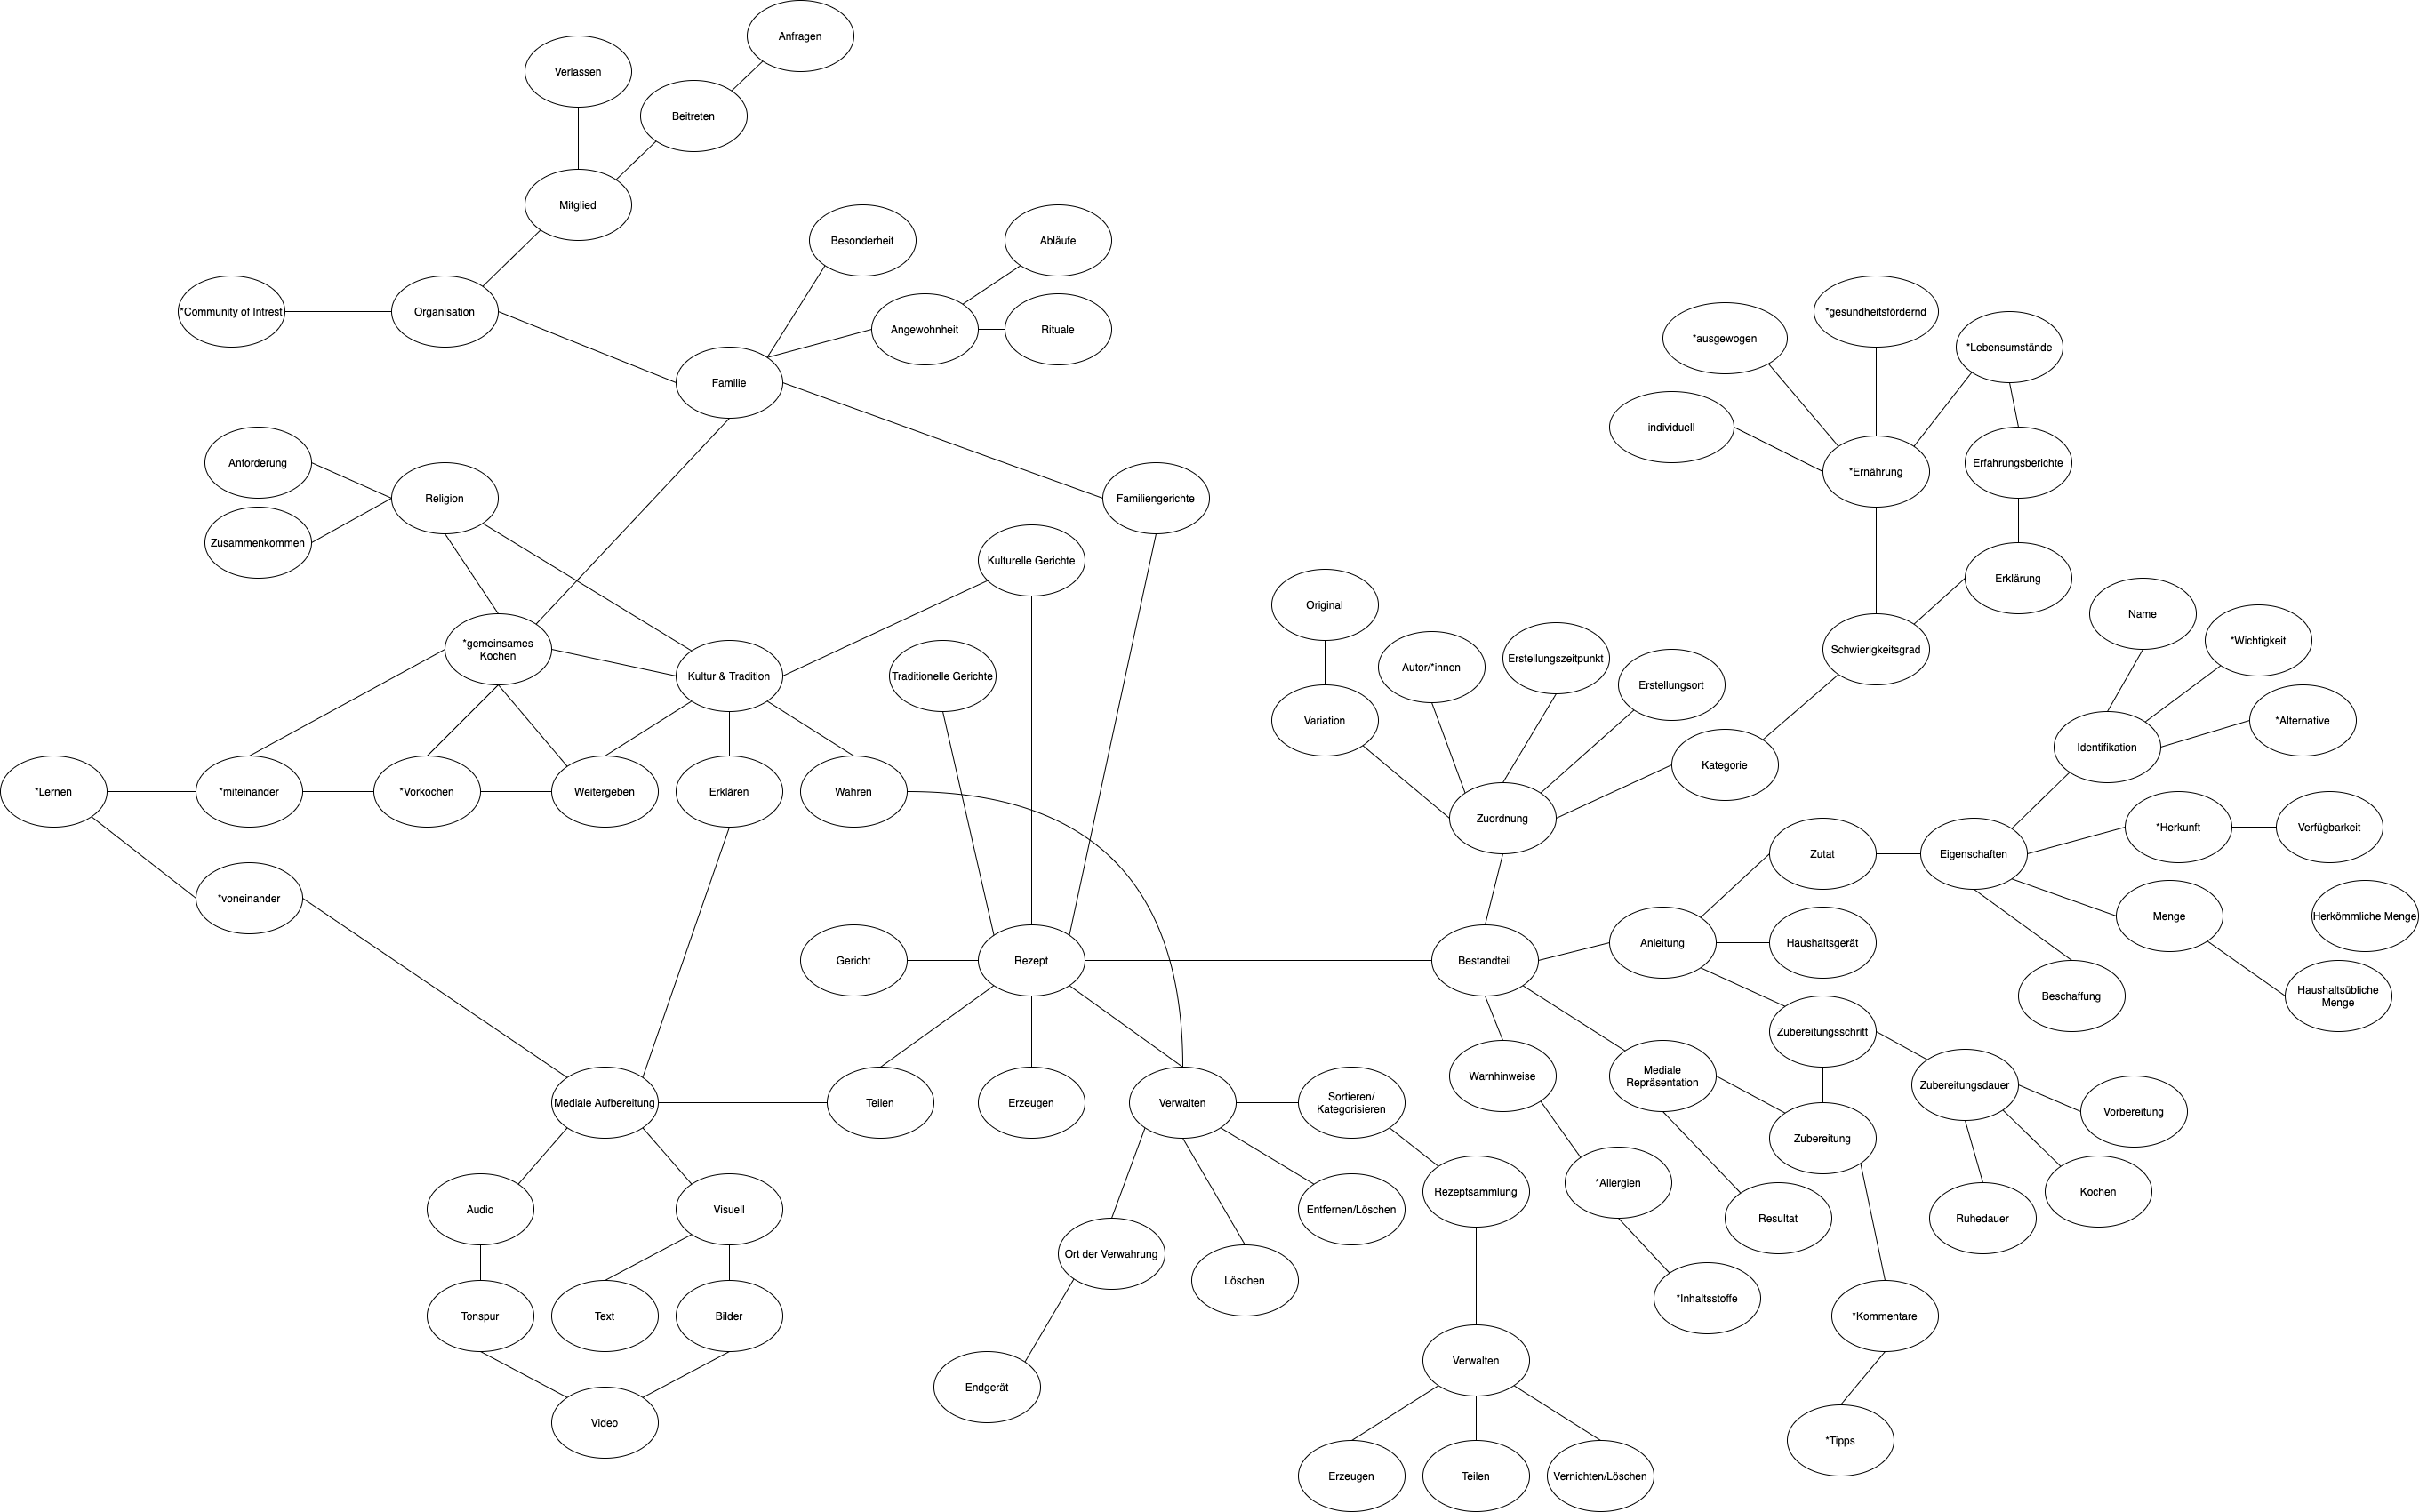
\includegraphics[width=1\textwidth]{../../Domänenmodell/PPSS21_Mai_Domänenmodell.png}
            \caption[Das Domänenmodell]{Domänenmodell, v1}
            \label{fig:domaenenmodell}
        \end{figure}
        Ergänzend zu dem Modell ist zu erwähnen, dass dieses Modell lediglich eine Momentaufnahme der gesamten Projektdomäne darstellt und sich im Laufe des Projekts durchaus noch verändern kann.

        \subsection{Problembeschreibung}\label{sec:Problembeschreibung}
        % Existenz und Beschreibung des Problemraums werden durch Quellen belegt
        
            \subsubsection{Kultur- und Traditions-Sharing}\label{sec:cultureandtradition}
            Um nicht eine weitere Plattform für den öffentlichen Austausch von Rezepten zu entwickeln, ist es unabdingbar, die Besonderheiten bei der Weitergabe von Kulturgut und tradionellen Rezepten zu erfassen und in die Systemarchitektur zu integrieren.\\
            So hat es sich durch User Stories ergeben, dass potentielle Nutzer die Funktion schätzen Anekdoten zu verfassen und Zutaten zu priorisieren, so wie, sofern notwendig, deren Herkunft anzugeben. Ein Beispiel dafür wäre die traditonelle Beschaffung von Pilzen aus einem nahegelegenen Wald. Diese Informationen sind oft mals privat und nur Familienmitgliedern mitzuteilen. Daher ergab sich des Weiteren auch eine Anforderung an die Weitergabe der Rezepte. \\
            Rezepte oder gar ganze Sammlungen, Kochbücher, müssen einzelnen Personen freigegeben werden können, beziehungsweise der Zugang angefragt werden können, ähnlich einer Freundschaftsanfrage auf sozialen Netzwerken. Daher ergibt es sich auch, dass diese Zugänge auch reversibel sein müssen.

            \subsubsection{Frontend}\label{sec:frontend}
            Abzuwägen war die Nutzung von nativen Applikationen\cite{netformic2020} oder der Nutzung webbasierter Anwendungen mit wesentlichem Fokus auf die Progressiven Web Applikationen (PWA), welche im Hinblick auf ihre Modernität und kommender Popularität\cite{netformic2020} durch aus attraktiv für die Umsetzung des Projekts sind. Auch der Vorteil einer PWA in Hinblick auf ihre Unabhängigkeit von Betriebssystemen, da der Service von möglichst vielen Familienmitgliedern genutzt, und auch über mehrere Generationen hinweg gepflegt werden soll.\cite{netformic2020} 

            \subsubsection{Systemarchitekturtyp}\label{sec:systemarchitecuretype}
            Es sind im wesentlichen zwei Systemarchitekturmodelle(siehe Figur \ref{fig:architecturstyles}) die die gesammelten Anforderungen erfüllen würden. Die Erste ist die Three-Tier-Architecture und die Zweite die Service-Oriented-Architecture mit möglicher Unterteilung in einzelne Microservices. Letzteres ist besonders attraktiv für Service die mit ihrer wachsenden Nutzerzahl auch deutlich mehr Leistung erfordern.
            \begin{figure}[hb] %!=overrides latex; h=here; t=top; b=bottom; p=special page for floating objects
                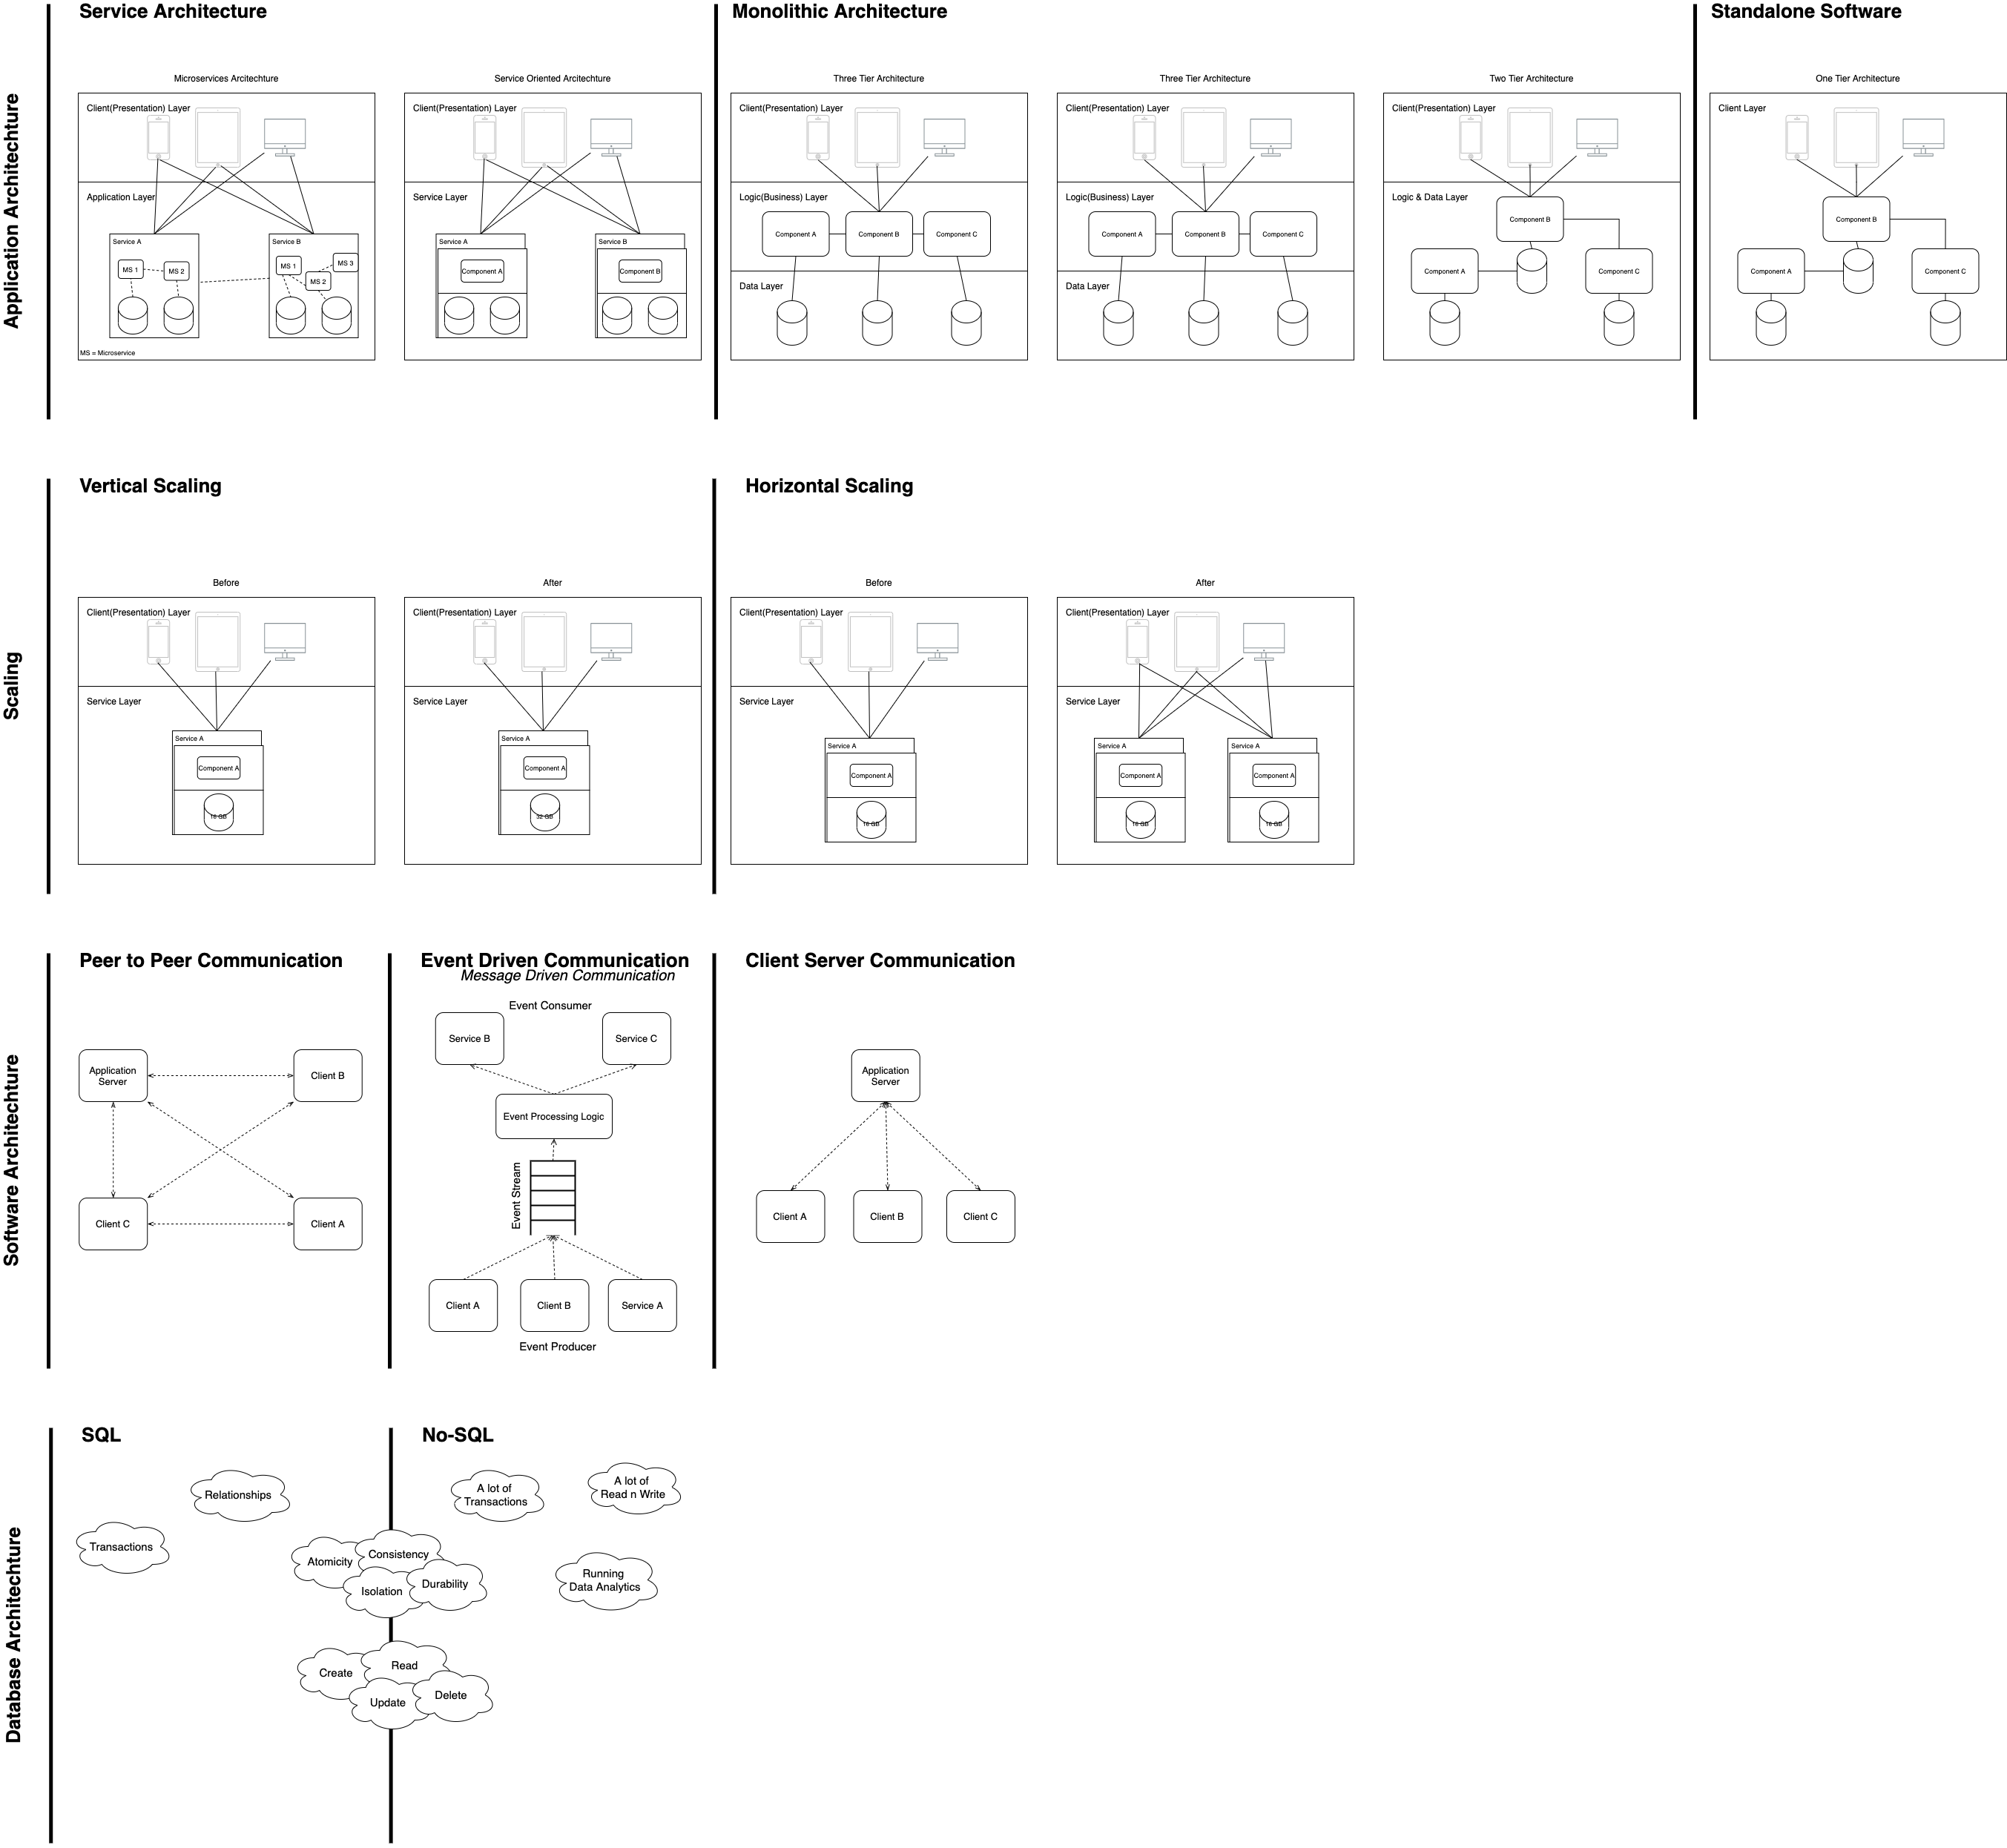
\includegraphics[width=1\textwidth]{../../Systemarchitektur/PPSS21_Mai_Architekturstile_gegenuebergestellt.png}
                \caption[Architekturstile]{Architekturstile, Modules}
                \label{fig:architecturstyles}
            \end{figure}

            \subsubsection{Kommunikationskanal}\label{sec:communicationchannel}
            Zu Beginn des Projekts war geplant die Kommunikation zwischen den einzelnen Nutzern von dem Server zu separieren und eine Peer to Peer Kommunikation(siehe Figur \ref{fig:architecturstyles}) zu implementieren. Diese hat aber zur Zeit noch ihre Schwächen, da hier immer noch ein Broker\cite{solance2012} benötigt wird um die einzelnen Peers zu verbinden und durch die dadurch resultierenden Daten auf Nutzerseite würde eine PWA auf Grund des begrenzt möglichen Speicherplatzes\cite{webdev2021} ungeeignet werden. Vorteile wie Offline Nutzbarkeit wurden zwar abgewägt, doch die Auswertung der User Stories und Interviews mit den potentiellen Nutzern ergaben kein Interesse an dieser Funktion. Wirklich gewünscht war die zuverlässige Kommunikation zwischen Server und Client(siehe Figur \ref{fig:architecturstyles}) und die Verschlüsselung der Daten auf der Server-Seite.

            \subsubsection{Datenbankform}\label{sec:databasetype}
            Im Wesentlichen stellt sich hier die Frage zwischen NoSQL oder SQL Datenbanken(siehe Figur \ref{fig:architecturstyles}). Auf Grund der dynamischen Inhalte im Frontend und dem vereinfachten Visualisieren von, in JSON formatierten, Datensätzen, bietet sich hier besonders NoSQL an. 

            \subsubsection{Datenschutz}\label{sec:privacy}
            Die Peer to Peer Kommunikation wurde von den potentiellen Nutzern als "unbequem" kommentiert. Daraus folgt, dass ein besonderer Fokus auf der Verschlüsselung der Daten, die Datenschutz konforme Verarbeitung/Speicherung der Daten und die sichere Übertragung gelegt werden muss. \\
            Die Zugangskontrolle stellt sich bisher als ein großes Problem heraus. Zur Zeit wurde noch keine effektive Lösung für dieses Problem gefunden. 
            

    \begin{figure}[h] %!=overrides latex; h=here; t=top; b=bottom; p=special page for floating objects
        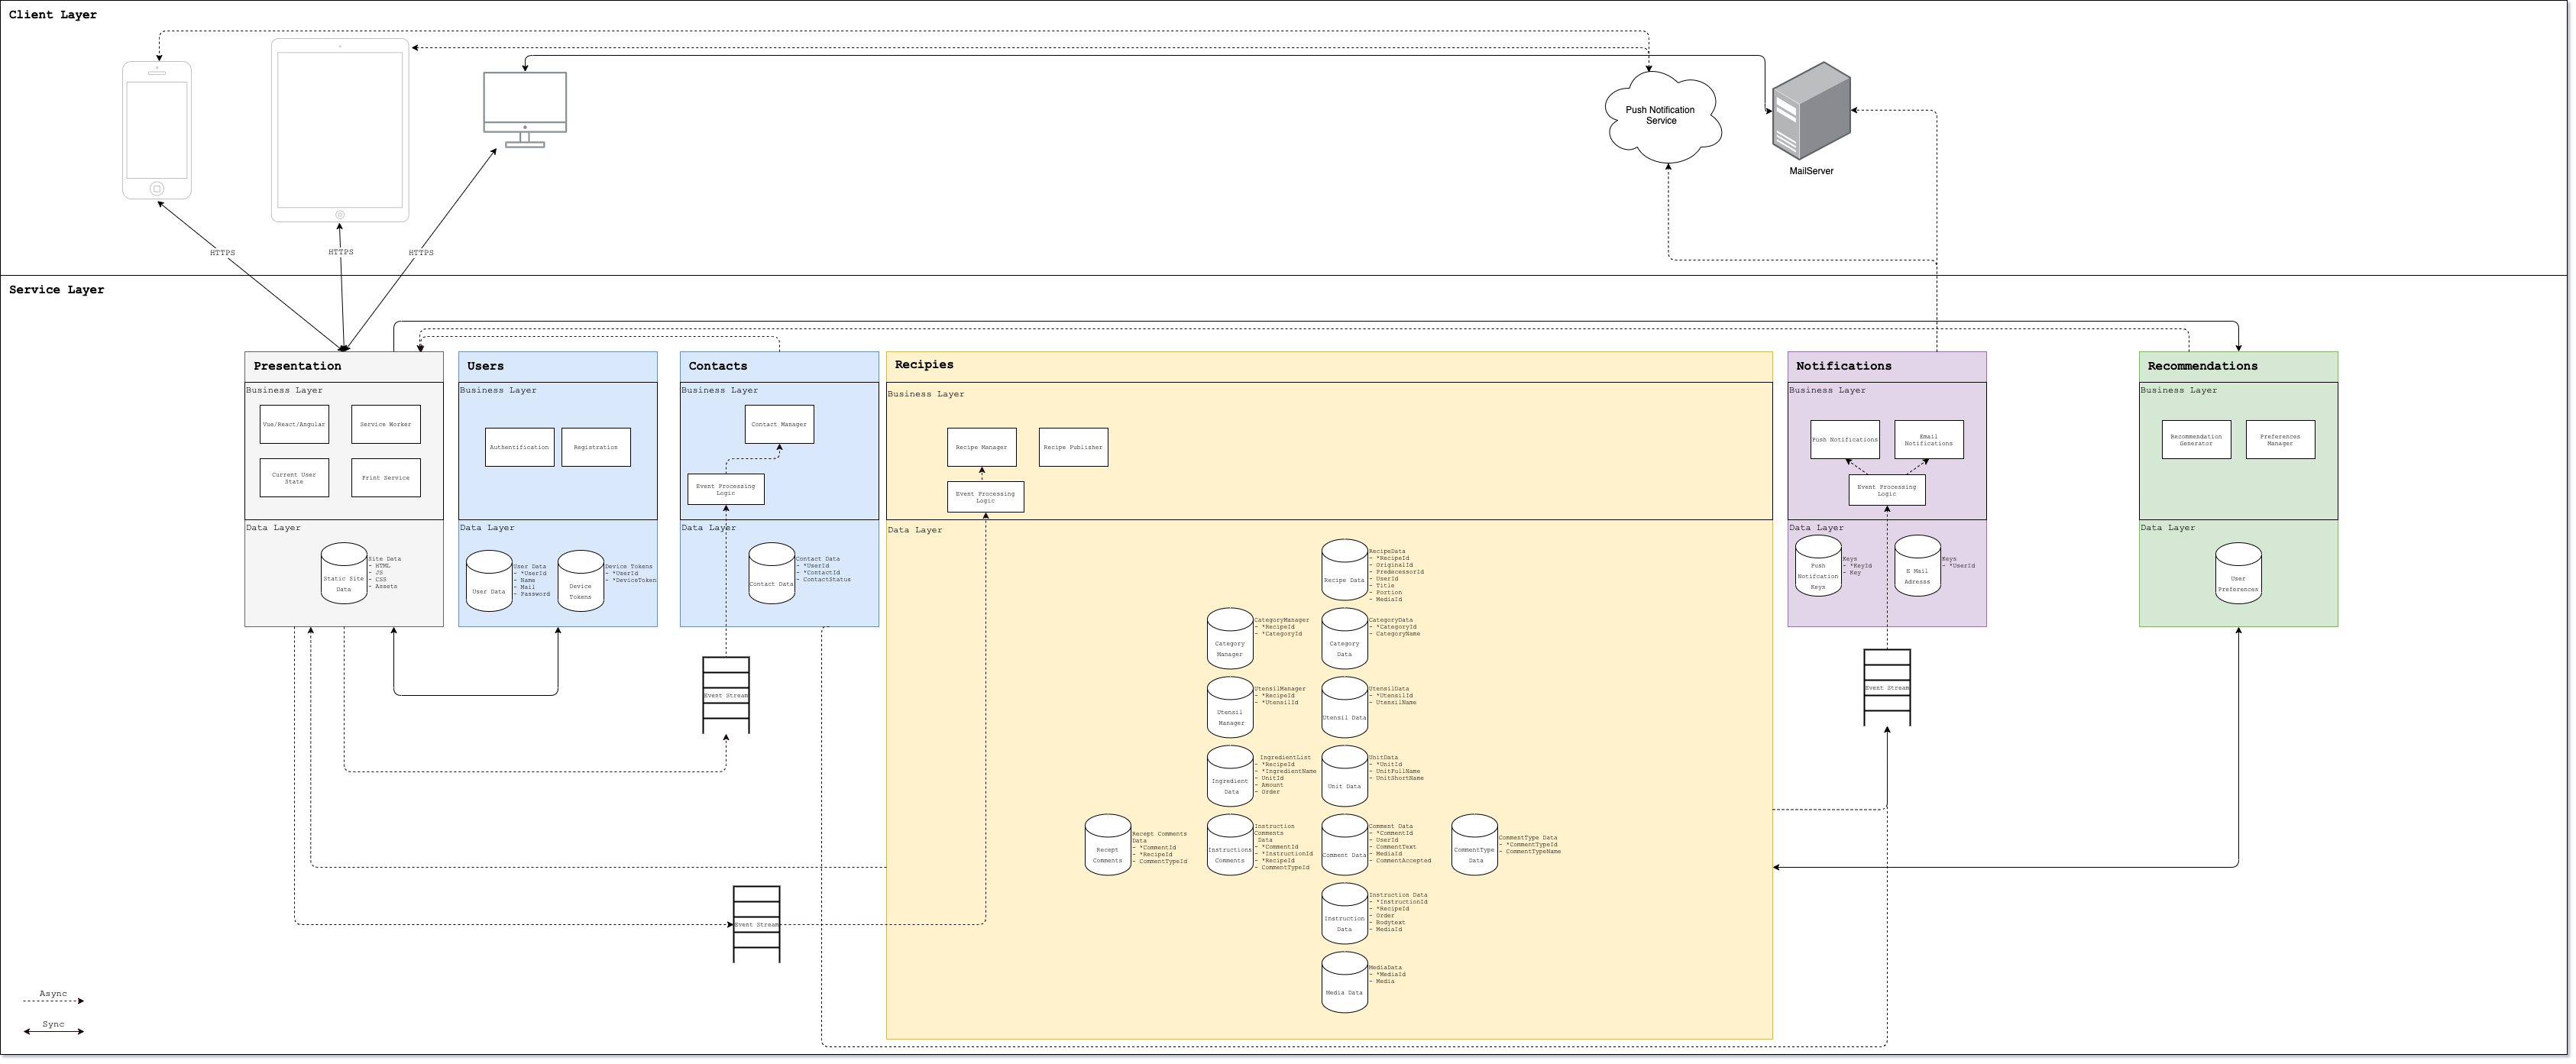
\includegraphics[width=1\textwidth]{../../Systemarchitektur/PPSS21_Mai_Systemarchitektur_v3.png}
        \caption[Die Vision]{Systemarchitekturmodell, v3}
        \label{fig:systemarchitekturmodell}
    \end{figure}
    \section{Zielsetzung und Vision}\label{sec:Zielsetzung}
    % Welchen Mehrwert bringt das Projekt und wie erreiche ich diesen?
    % Die Vision ist in der Regel technologieunabhängig; außer sie sind aus dem Problemraum heraus begründet
    % Was soll warum behandelt werden?
    Der Mehrwert des Projekts liegt in dem Vereinfachten Austausch über Traditionen und Kulturgut im Rahmen des Kochens innerhalb einer Familie. Die Förderung neuartiger Technologien und Design Patterns wie PWA und Service Oriented Architechure sind dabei nicht unerheblich.\\
    Am Ende des Projekts soll ein einfach zugänglicher Service für jeden Nutzer erreichbar gemacht werden. \\
    Der Service umfasst die Funktionalitäten:
    \begin{itemize}
        \item Online-Speicherung von Rezepten in einer verschlüsselten Datenbank
        \item Ergonomisches Erstellen und Interagieren mit Rezepten
        \item Zugriffskontrolle auf die eigene Sammlung und oder einzelner Rezepte
        \item Soziale Interaktion und die Dokumentation von Erfahrungen sowie Anekdoten zu Rezepten
        \item Exportierung als PDF oder Druckvorlage und Importierung von Rezepten aus Externen Quellen
    \end{itemize} 

    \section{Relevanz}\label{sec:Relevanz}
    % Inwiefern ist die Adressierung dieser bestimmten Problemstellung mittels dieser bestimmen Zielsetzung relevant?

        \subsection{Gesellschaftliche Relevanz}\label{sec:Gesellschaftliche}
        % gesellschaftliche Relevanz: trägt zur öko-sozialen Transformation bei
        Mit dem Serice soll der Zusammenhalt und die Kommunikation innerhalb der Familien angeregt und nachhaltig unterstützt werden. Trationen und Kultur sollen nicht mit der Zeit verloren gehen, sondern gezielt weitergegeben werden können. Gleichzeitig bietet das ausführliche Dokumentieren der eigenen Rezepte auch die Möglichkeit, der eigenen Kultur Fremde für die Eigene zu begeistern und mit dieser zu konfrontieren.

        \subsection{Wirtschaftliche Relevanz}\label{sec:Wirtschaftliche}
        % wirtschaftliche Relevanz: z.B. schließt eine Marktlücke, unterstützt innovative Geschäftsmodelle,
        Bereits bestehende Plattformen bieten viele der Funktionen, die sich mit den im Projekt erarbeiteten Nutzeranforderungen decken, doch bleibt der Bedarf nach einer Plattform mit dem Fokus auf die eigenen Nutzer und dem Teilen der Inhalte mit exklusiven Nutzern bislang ungedeckt.

        \subsection{Wissenschaftliche Relevanz}\label{sec:Wissenschaftliche}
        % wissenschaftliche Relevanz: bringt einen wissens-orientierten Mehrwert
        Das Weiterentwickeln von PWA's und den verteilten Systemen wird absehbar noch Thema der Webentwickler bleiben, und das erarbeiten eines solchen Services kann für mehr Aufmerksamkeit für die Technologie sorgen. An den Weiterentwicklungen würden mehr Entwickler profitieren.

    \section{Persönliche Motivation}\label{sec:Motivation}
    Seit nun mehr als einem Jahr beschäftige ich mich mit dem Thema. Ich halte das Thema der Ernährung, sowie den Schutz von Familienkultur und Traditionen auch im Hinblick auf Religion für wichtig, da durch zunehmende Globalisierung und dem Übernehmen von Restaurant-Ketten, die lokalen Geschäfte verdrengt werden. \\
    Daher möchte ich eine ergonomische Möglichkeit für alle Gruppen entwickeln, ihre Geschichte zu dokumentieren und zu wahren. Damit auch kommende Generationen ihre eigene Kultur entdecken können. \\
    Ich plane Funktionalitäten wie Empfehlungen für die eigene Ernährung mit Hilfe von analytischen Algorithmen, basierend auf den Familienrezepten, zu entwickeln. \\
    Ich hoffe Sie teilen meine Begeisterung.

    \newpage
    % Bibliothek einbinden
    \bibliographystyle{plain} 
    \bibliography{mai-joel-maximilian-pp-ss-2021.bib}

\end{document}